\documentclass{beamer}
\usepackage[utf8]{inputenc}
\usepackage{amsmath}

\usetheme{Madrid}
\usecolortheme{beaver}

\title{Rayo de Electrones: Bitácora de Laboratorio}
\author{Sebastian Rodríguez, Laura Torres, Julian Avila}
\institute{Universidad Distrital Francisco José de Caldas}
\date{\today}

\begin{document}

\begin{frame}
  \titlepage
\end{frame}

%------------------------------------------------
\begin{frame}{Objetivo del Montaje Experimental}
  \begin{block}{Meta Principal}
    Demostrar la deflexión de un haz de electrones bajo la influencia de campos magnéticos generados por pares de bobinas de Helmholtz.
  \end{block}
  \vspace{1cm}
  \begin{itemize}
    \item Estudiar la dinámica del haz en configuraciones de campo uniforme y de gradiente.
    \item Analizar las figuras resultantes en una pantalla fluorescente.
    \item Comparar los resultados experimentales con las predicciones teóricas del electromagnetismo clásico.
  \end{itemize}
\end{frame}

%------------------------------------------------
\begin{frame}{Componentes Clave del Montaje}
  \begin{itemize}
    \item \textbf{Cañón de Electrones (Leibold):}
      \begin{itemize}
        \item Genera un haz de electrones colimado.
        \item Potencial de aceleración: $V_{acc} \approx 3.1 \, \text{kV} - 4.3 \, \text{kV}$.
      \end{itemize}
    \item \textbf{Tubo de Rayos Catódicos (Leibold):}
      \begin{itemize}
        \item Cámara de vacío donde viaja el haz de electrones.
      \end{itemize}
    \item \textbf{Pares de Bobinas de Helmholtz (Leibold):}
      \begin{itemize}
        \item Dos pares coaxiales alimentados por fuentes de corriente variable ($I \le 2 \, \text{A}$).
        \item Parámetros aproximados: Radio $R \approx 6.5 \, \text{cm}$, número de vueltas por bobina $N \approx 320$.
      \end{itemize}
    \item \textbf{Fuentes de Corriente Variable:}
      \begin{itemize}
        \item Controlan la magnitud del campo magnético ($I \le 3 \, \text{A}$).
      \end{itemize}
    \item \textbf{Pantalla Fluorescente:}
      \begin{itemize}
        \item Visualiza la trayectoria y deflexión del haz.
      \end{itemize}
  \end{itemize}
\end{frame}

%------------------------------------------------
\begin{frame}{Disposición Experimental}
  \begin{figure}
    \centering
    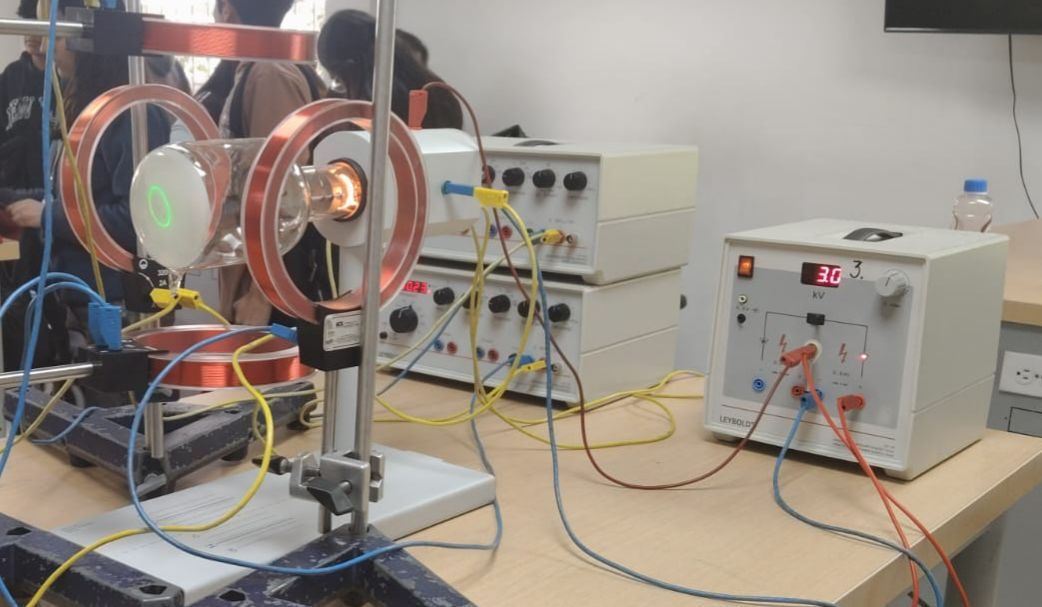
\includegraphics[width=0.7\textwidth]{../Figures/Montaje.jpeg}
    \caption{Montaje experimental.}
  \end{figure}
  \begin{itemize}
    \item El cañón de electrones se alinea para que el haz pase por el centro de las bobinas de Helmholtz.
    \item Los dos pares de bobinas son coaxiales, con su eje coincidiendo con la trayectoria inicial del haz.
  \end{itemize}
\end{frame}

%------------------------------------------------
\begin{frame}{Configuraciones de Bobinas y Campo Magnético}
  \begin{block}{1. Configuración de Helmholtz (Campo Aditivo)}
    \begin{itemize}
      \item \textbf{Descripción:} La corriente fluye en la misma dirección en ambas bobinas de un par.
      \item \textbf{Campo Magnético:} Produce un campo $\vec{B}$ uniforme y aditivo en la región central, paralelo al eje.
      \item \textbf{Efecto en el Haz:} Un campo uniforme perpendicular a la velocidad $\vec{v}$ del electrón causa una deflexión circular, gobernada por la fuerza de Lorentz $\vec{F}_L = q(\vec{v} \times \vec{B})$.
    \end{itemize}
  \end{block}
\end{frame}
\begin{frame}
  \begin{block}{2. Configuración Anti-Helmholtz (Campo de Gradiente)}
    \begin{itemize}
      \item \textbf{Descripción:} La corriente se invierte en una de las bobinas del par.
      \item \textbf{Campo Magnético:} Crea un campo con un fuerte gradiente ($\nabla \vec{B}$) en la región central. El campo es nulo en el punto medio.
      \item \textbf{Efecto en el Haz:} Genera fuerzas variables, resultando en patrones de deflexión complejos y efectos de enfoque/desenfoque.
    \end{itemize}
  \end{block}
\end{frame}

%------------------------------------------------
\begin{frame}{Funcionamiento y Observaciones Iniciales}
  \begin{itemize}
    \item Las fuentes de corriente variable permiten ajustar la magnitud del campo magnético.
    \item Se aplicaron señales de corriente sinusoidales, de rampa y cuadradas, con frecuencias $f \le 100 \, \text{Hz}$.
    \item La interacción del haz de electrones con el campo magnético resultante produjo patrones luminosos en la pantalla.
    \item Se observaron figuras dinámicas, semejantes a las figuras de Lissajous pero con variaciones temporales debidas a la modulación del campo magnético.
  \end{itemize}
\end{frame}

%------------------------------------------------
\begin{frame}{Análisis de la Interacción de Espín (Justificación de su Descarte)}
  El electrón, como partícula cuántica con espín $s=1/2$, posee un momento dipolar magnético intrínseco $\vec{\mu}$. Esto podría generar una fuerza adicional si el campo magnético no es uniforme. La fuerza de Stern-Gerlach es $\vec{F}_{spin} = \nabla(\vec{\mu} \cdot \vec{B})$.

  \begin{alertblock}{Conclusión}
    Esta fuerza es despreciable por dos razones fundamentales.
  \end{alertblock}
\end{frame}

\begin{frame}
  \begin{columns}[T]
    \begin{column}{0.5\textwidth}
      \textbf{1. Comparación de Magnitudes}
      \begin{itemize}
        \item En campos uniformes (Helmholtz), $\nabla \vec{B} = 0$, por lo que $\vec{F}_{spin} \equiv 0$.
        \item En campos de gradiente (Anti-Helmholtz), el cociente de fuerzas es:
          $$ \frac{|\vec{F}_{spin}|}{|\vec{F}_{Lorentz}|} \approx 10^{-11} $$
          La fuerza de Lorentz es 11 órdenes de magnitud mayor.
      \end{itemize}
    \end{column}
    \begin{column}{0.5\textwidth}
      \textbf{2. Efecto de la Precesión de Larmor}
      \begin{itemize}
        \item El momento magnético $\vec{\mu}$ precesa alrededor de la dirección de $\vec{B}$ con la frecuencia de Larmor $\omega_L$.
        \item La fuerza $\vec{F}_{spin}$ depende de la orientación instantánea de $\vec{\mu}$ y, por lo tanto, oscila rápidamente.
        \item El efecto neto de esta fuerza oscilante sobre la trayectoria macroscópica se promedia a cero.
      \end{itemize}
    \end{column}
  \end{columns}
  \textbf{Conclusión:} Es físicamente justificable y computacionalmente necesario ignorar la interacción de espín y tratar al electrón como una carga clásica.
\end{frame}

%------------------------------------------------
\begin{frame}{Resultados: Campo Uniforme (Configuración Helmholtz)}
  \begin{block}{Observaciones}
    Se generaron trayectorias cerradas y estables en la pantalla, conocidas como \textbf{figuras de Lissajous}.
  \end{block}

  \begin{itemize}
    \item \textbf{Validación:} La topología de estas figuras se correlacionó directamente con los parámetros de control de las corrientes de alimentación.
    \item El cociente de frecuencias enteras ($\omega_1 / \omega_2$) determinó el número de lóbulos a lo largo de cada eje.
    \item La diferencia de fase ($\phi$) controló la apertura y simetría de la trayectoria, transicionando desde líneas diagonales ($\phi=0$) a elipses o círculos ($\phi=\pi/2$).
  \end{itemize}
\end{frame}

\begin{frame}
  \begin{alertblock}{Confirmación}
    Esta correspondencia directa validó el modelo de campo uniforme como una excelente aproximación para describir la dinámica macroscópica del haz en campos cruzados.
  \end{alertblock}
\end{frame}

%------------------------------------------------
\begin{frame}{Resultados: Campo de Gradiente (Configuración Anti-Helmholtz)}
  \begin{block}{Observaciones}
    Se produjeron patrones radiales. El haz no trazaba una curva, sino que convergía a un punto central y se expandía hacia afuera periódicamente.
  \end{block}

  \begin{itemize}
    \item Se observó una \textbf{pulsación rítmica} del haz.
    \item El radio máximo del patrón circular en la pantalla fue proporcional a la amplitud de la corriente.
    \item La frecuencia de pulsación coincidió con la frecuencia de alimentación de la corriente.
  \end{itemize}

  \begin{alertblock}{Confirmación}
    Este comportamiento es una manifestación visual directa del efecto de \textbf{enfoque} (colapso del haz) y \textbf{desenfoque} (expansión) predicho por el modelo cuadrupolar, confirmando la capacidad de estos campos para manipular la sección transversal del haz.
  \end{alertblock}
\end{frame}

%------------------------------------------------
\begin{frame}{Resultados: Configuración Mixta y División del Haz}
  \begin{block}{Configuración Híbrida}
    Un par de bobinas en modo Helmholtz (campo uniforme $\vec{B}_x$) y el otro en modo Anti-Helmholtz (campo de gradiente $\nabla B_y$).
  \end{block}

\end{frame}

\begin{frame}

  \begin{alertblock}{Resultado Más Sorprendente}
    El haz de electrones, en lugar de curvarse o expandirse, \textbf{osciló de forma estable entre dos posiciones discretas y bien definidas}. Parecía como si la pantalla presentara dos atractores estables para la trayectoria.
  \end{alertblock}

  \begin{itemize}
    \item \textbf{Semejanza Visual:} Esta división del haz evoca visualmente el patrón obtenido en el histórico experimento de Stern-Gerlach.
    \item \textbf{Distinción Crucial:} Sin embargo, es fundamental enfatizar que la física subyacente \textbf{no corresponde a una separación de estados de espín}.
    \item \textbf{Mecanismo Postulado:} La compleja topología del campo magnético mixto probablemente crea un potencial con dos mínimos locales, guiando al haz a saltar entre estas dos trayectorias estables a la frecuencia de los campos.
  \end{itemize}
\end{frame}

%------------------------------------------------
\begin{frame}{Discusión: ¿Análogo Clásico vs. Efecto Cuántico?}
  \begin{block}{Análisis Riguroso}
    El fenómeno observado es un fascinante análogo clásico del experimento de Stern-Gerlach (SG), pero es de naturaleza puramente clásica y no debe ser categorizado como un efecto SG.
  \end{block}

  Analizaremos tres diferencias fundamentales:
  \begin{enumerate}
    \item Naturaleza de la Fuerza Dominante
    \item Campos Dinámicos (AC) vs. Estáticos (DC)
    \item Separación Clásica vs. Cuantizada
  \end{enumerate}
\end{frame}

%------------------------------------------------
\begin{frame}{Discusión 1: Naturaleza de la Fuerza Dominante}
  \begin{block}{Experimento SG Original}
    \begin{itemize}
      \item Utiliza partículas \textbf{neutras} (e.g., átomos de plata) para aislar la interacción entre el momento dipolar magnético y el gradiente de campo.
      \item La fuerza responsable de la separación es la fuerza de Stern-Gerlach: $\vec{F}_{SG} = \nabla(\vec{\mu} \cdot \vec{B})$.
    \end{itemize}
  \end{block}

\end{frame}

\begin{frame}

  \begin{block}{Nuestro Experimento}
    \begin{itemize}
      \item La partícula es un \textbf{electrón}, que tiene carga $e$.
      \item Como se demostró cuantitativamente, la fuerza de Lorentz que actúa sobre la carga del electrón es aproximadamente $10^{11}$ veces mayor que cualquier posible fuerza sobre su espín.
        $$ |\vec{F}_{Lorentz}| \gg |\vec{F}_{spin}| $$
      \item \textbf{Conclusión:} La dinámica observada es resultado casi exclusivo de la fuerza de Lorentz. La división no se origina por una interacción de espín.
    \end{itemize}
  \end{block}
\end{frame}

%------------------------------------------------
\begin{frame}{Discusión 2: Campos Dinámicos (AC) vs. Estáticos (DC)}
  \begin{block}{Experimento SG Canónico}
    \begin{itemize}
      \item Requiere un campo magnético \textbf{estático (DC)} con un gradiente espacial muy pronunciado y constante en el tiempo.
      \item La separación producida es, por tanto, \textbf{estática}: los átomos se desvían permanentemente hacia una de dos trayectorias.
    \end{itemize}
  \end{block}

\end{frame}


\begin{frame}

  \begin{block}{Nuestro Montaje}
    \begin{itemize}
      \item Se basa fundamentalmente en campos \textbf{dinámicos (AC)} que oscilan a una frecuencia de $f \approx 50-60 \, \text{Hz}$.
      \item El patrón observado no es una separación estática, sino una \textbf{oscilación} del haz entre dos puntos.
      \item El electrón no elige una de dos trayectorias fijas; es guiado alternativamente a una posición y luego a la otra por los campos variables en el tiempo.
    \end{itemize}
  \end{block}
\end{frame}

%------------------------------------------------
\begin{frame}{Discusión 3: Separación Clásica vs. Cuantizada}
  \begin{block}{Separación en el Experimento SG}
    \begin{itemize}
      \item Es una manifestación directa de la \textbf{cuantización del espacio}.
      \item Para una partícula de espín-1/2, solo existen dos proyecciones de espín posibles ($\pm \hbar/2$), resultando en exactamente dos haces.
      \item La magnitud de esta separación depende de constantes fundamentales.
    \end{itemize}
  \end{block}

\end{frame}

\begin{frame}

  \begin{block}{Separación en Nuestro Experimento}
    \begin{itemize}
      \item La posición de los dos puntos observados \textbf{no está fijada por constantes fundamentales}.
      \item Depende de parámetros \textbf{clásicos y continuamente ajustables}: geometría de la bobina, amplitud y frecuencia de la corriente, y energía inicial del haz.
      \item Se postula que la topología del campo mixto crea un \textbf{potencial efectivo con dos mínimos locales}. La posición de estos mínimos puede modificarse alterando voltajes y corrientes, lo cual sería imposible en una verdadera división cuántica.
    \end{itemize}
  \end{block}
\end{frame}

%------------------------------------------------
\begin{frame}{Conclusión}
  \begin{alertblock}{Fenómeno Observado}
    El fenómeno de división del haz es un extraordinario \textbf{análogo clásico} del experimento de Stern-Gerlach.
  \end{alertblock}

  \begin{itemize}
    \item Demuestra cómo la ingeniería compleja de campos electromagnéticos clásicos y dependientes del tiempo puede generar un comportamiento que simula visualmente un resultado cuántico.
    \item Lejos de ser una medida de espín, es un testimonio de la riqueza de la \textbf{dinámica no lineal en el electromagnetismo clásico}.
    \item La "división" es una oscilación forzada entre dos puntos de estabilidad dinámica, controlados por parámetros externos, y no una manifestación de la cuantización del momento angular intrínseco.
  \end{itemize}
\end{frame}

\end{document}
